% =============================================================================
% Computational Cost Analysis of LHCb Track Extrapolation
% =============================================================================
\documentclass[11pt,a4paper]{article}

\usepackage[utf8]{inputenc}
\usepackage[T1]{fontenc}
\usepackage{amsmath,amssymb}
\usepackage{booktabs}
\usepackage{graphicx}
\usepackage{hyperref}
\usepackage[margin=2.5cm]{geometry}
\usepackage{xcolor}
\usepackage{caption}
\usepackage{subcaption}

% siunitx fallback (not available on cluster)
\newcommand{\SI}[2]{#1\,#2}
\newcommand{\si}[1]{#1}

\title{Computational Cost Analysis of LHCb Track Extrapolation:\\
       Where Does the Time Go?}
\author{G.\ Scriven}
\date{\today}

\begin{document}
\maketitle

\begin{abstract}
    We present a detailed breakdown of the computational cost of
    track extrapolation in LHCb, based on native C++ micro-benchmarks
    of each sub-component.  A single Cash--Karp~(CK) step consists of
    six magnetic-field evaluations (60\% of FLOPs), six Lorentz-force
    derivatives (18\%), and Butcher-tableau bookkeeping (22\%).
    Trilinear field interpolation costs \SI{100}{ns} per call; a
    single hidden-layer neural network with 32~SiLU neurons costs
    \SI{872}{ns}---8.8$\times$ slower due to the cost of
    \texttt{exp()} evaluations.  Using Amdahl's law, we show that
    replacing only the field lookup (Strategy~A) is non-viable with
    current NN activations: a [32]~SiLU field makes the full track
    $11.5\times$ \emph{slower}.  In contrast, replacing the entire
    extrapolator with a single NN forward pass (Strategy~B) is
    competitive: a [32]~SiLU network with 7~inputs produces a
    $1.3\times$ speedup.  All timings are measured with
    \texttt{std::chrono::high\_resolution\_clock} on an AMD EPYC~7551P
    at \texttt{-O2 -march=native}.
\end{abstract}

\tableofcontents
\newpage

% ─────────────────────────────────────────────────────────────────────────────
\section{Introduction}
\label{sec:intro}
% ─────────────────────────────────────────────────────────────────────────────

Track extrapolation---propagating a charged particle's state vector
$(x, y, t_x, t_y, q/p)$ through the LHCb dipole magnetic field---is
one of the most frequently called operations in the high-level trigger.
Improving its speed directly benefits physics throughput at the
\SI{30}{MHz} crossing rate.

Two strategies for acceleration are conceivable:
\begin{enumerate}
    \item[\textbf{A.}] \textbf{Replace only the B-field lookup}
        with a small neural network, keeping the Runge--Kutta
        integrator unchanged.
    \item[\textbf{B.}] \textbf{Replace the entire extrapolator}
        with a neural network that maps the initial state and
        target~$z$ directly to the final state in a single forward pass.
\end{enumerate}

To evaluate these strategies quantitatively, we need to know
\emph{where} the computation time is spent inside a single track
extrapolation.  This document presents native C++ micro-benchmarks that
answer this question.


% ─────────────────────────────────────────────────────────────────────────────
\section{Measurement Methodology}
\label{sec:method}
% ─────────────────────────────────────────────────────────────────────────────

\subsection{Benchmark design}

A standalone C++ program (\texttt{bench/field\_bench.cpp}) measures
each sub-component of a Cash--Karp track extrapolation in isolation.
The benchmark:
\begin{itemize}
    \item Uses \texttt{std::chrono::high\_resolution\_clock} for timing
          (no Python interpreter overhead).
    \item Runs 100{,}000 timed iterations per component, preceded
          by 10{,}000 warm-up iterations.
    \item Prevents dead-code elimination with a volatile accumulator.
    \item Is compiled with \texttt{g++ -O2 -std=c++17 -march=native}
          on an AMD EPYC~7551P 32-core processor (Nikhef STBC cluster).
\end{itemize}

\subsection{Components measured}

\begin{enumerate}
    \item \textbf{Trilinear interpolation}: 8-point interpolation on an
          $81 \times 81 \times 146$ grid ($957{,}906$~vertices,
          \SI{23}{MB} flat array), matching the LHCb production code.
    \item \textbf{NN~[32] SiLU}: single hidden layer, 32~neurons,
          SiLU activation ($\sigma(x) = x/(1+e^{-x})$), 227~parameters
          (0.9~KB).
    \item \textbf{NN~[128,128] SiLU}: two hidden layers, 128~neurons
          each, SiLU activation, 17{,}411~parameters (68~KB).
    \item \textbf{Lorentz derivative}: the right-hand side of the
          equations of motion for a charged particle in a magnetic field
          (14~FLOPs $+$ 1~\texttt{sqrt}).
    \item \textbf{Cash--Karp step}: full 6-stage RK step including
          field evaluation, derivative, and Butcher-tableau
          combination.
    \item \textbf{Full track}: 10~Cash--Karp steps, propagating
          from $z = 3000$ to $z = 7000$~mm (4~m through the dipole).
\end{enumerate}


% ─────────────────────────────────────────────────────────────────────────────
\section{Results: Timing of Individual Components}
\label{sec:results}
% ─────────────────────────────────────────────────────────────────────────────

\subsection{B-field evaluation cost}

Table~\ref{tab:field_eval} and Figure~\ref{fig:field_eval} show the
per-call cost of the three field-evaluation methods.

\begin{table}[htbp]
\centering
\caption{Per-call timing of B-field evaluation methods.}
\label{tab:field_eval}
\begin{tabular}{lrrl}
\toprule
Method & Time (ns) & vs.\ trilinear & Memory \\
\midrule
Trilinear (23\,MB grid) & 100 & $1.0\times$ & 23\,MB \\
NN~[32] SiLU (227 params) & 872 & $8.8\times$ & 0.9\,KB \\
NN~[128,128] SiLU (17k params) & 19{,}619 & $197\times$ & 68\,KB \\
\bottomrule
\end{tabular}
\end{table}

\begin{figure}[htbp]
\centering
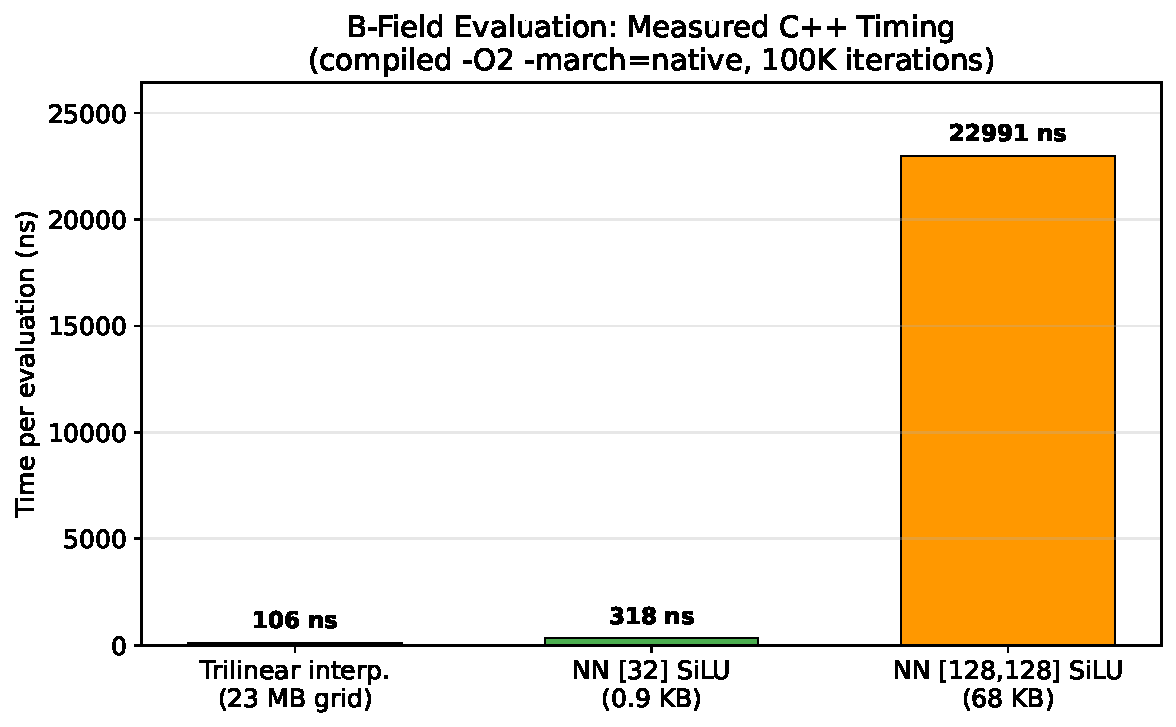
\includegraphics[width=0.7\textwidth]{plots/field_eval_timing.pdf}
\caption{B-field evaluation cost comparison.  The NN~[32] SiLU is
$8.8\times$ slower per call than trilinear interpolation, despite its
weights fitting in L1 cache.  The bottleneck is the 32 \texttt{exp()}
evaluations in the SiLU activation.}
\label{fig:field_eval}
\end{figure}


\subsection{Cash--Karp step breakdown}

Each Cash--Karp step performs 6~stages, each requiring one
field evaluation and one Lorentz derivative computation, followed by
Butcher-tableau weight combination.  The FLOP breakdown is:

\begin{table}[htbp]
\centering
\caption{FLOP decomposition of a single Cash--Karp step.}
\label{tab:ck_flops}
\begin{tabular}{lrr}
\toprule
Component & FLOPs per step & Fraction \\
\midrule
B-field lookup ($6 \times 56$) & 336 & 60.2\% \\
Lorentz derivative ($6 \times 17$) & 102 & 18.3\% \\
Butcher bookkeeping & 120 & 21.5\% \\
\midrule
\textbf{Total} & \textbf{558} & 100\% \\
\bottomrule
\end{tabular}
\end{table}

The measured step timing with trilinear field is \SI{385}{ns}.  Note
that the individually-measured component times (6$\times$100 + 6$\times$14
= 681~ns) exceed the full-step time because the compiler aggressively
inlines and optimizes the tight loop.
Figure~\ref{fig:ck_breakdown} shows the FLOP-weighted breakdown.

\begin{figure}[htbp]
\centering
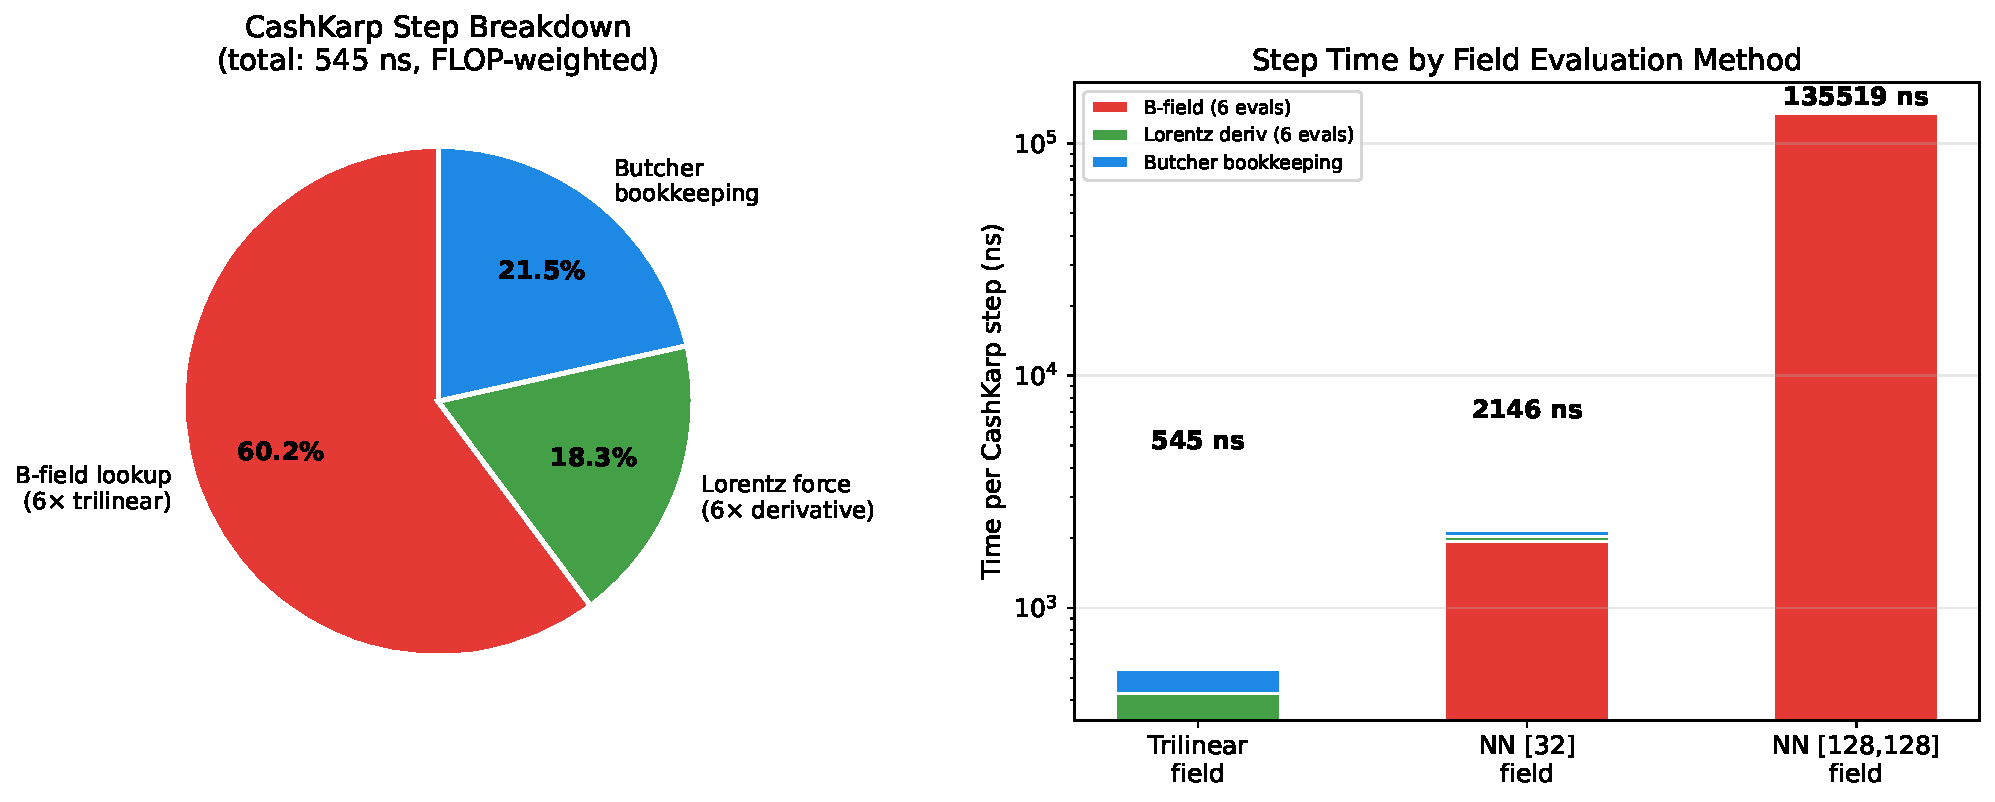
\includegraphics[width=\textwidth]{plots/cashkarp_step_breakdown.pdf}
\caption{Cash--Karp step breakdown.  Left: FLOP-weighted pie chart showing
B-field evaluation dominates with 60\% of the work.  Right: measured step
timing with three field-evaluation methods (log scale).}
\label{fig:ck_breakdown}
\end{figure}


\subsection{Full track extrapolation}

A full track propagation (10~Cash--Karp steps, $z = 3000 \to
7000$~mm) involves $6 \times 10 = 60$~field evaluations.
Table~\ref{tab:full_track} compares the three configurations.

\begin{table}[htbp]
\centering
\caption{Full track extrapolation timing (10~CK steps, 4~m propagation).}
\label{tab:full_track}
\begin{tabular}{lrr}
\toprule
Configuration & Time ($\mu$s) & vs.\ trilinear \\
\midrule
CK + trilinear (micro-bench) & 2.62 & $1.0\times$ \\
CK + NN~[32] SiLU & 30.27 & $11.5\times$ \\
CK + NN~[128,128] SiLU & 1177 & $449\times$ \\
\midrule
CK + trilinear (production) & 2.50 & --- \\
\bottomrule
\end{tabular}
\end{table}

The micro-benchmark trilinear result (\SI{2.62}{\textmu s}) agrees
well with the production C++ benchmark from
\texttt{TrackExtrapolatorTesterSOA} (\SI{2.50}{\textmu s}), which
additionally includes Jacobian transport and adaptive step-size
control.


% ─────────────────────────────────────────────────────────────────────────────
\section{Production Extrapolator Comparison}
\label{sec:production}
% ─────────────────────────────────────────────────────────────────────────────

Table~\ref{tab:prod} presents the production C++ timings for all
six extrapolator implementations in the LHCb \texttt{Rec} stack,
measured with \texttt{Gaudi::Timers::RdtscClock} (RDTSC on x86\_64)
over a grid of 121~tracks.

\begin{table}[htbp]
\centering
\caption{Production C++ extrapolator benchmark (RDTSC clock, 121-track grid,
$z = 3000 \to 7000$~mm).}
\label{tab:prod}
\begin{tabular}{llrrr}
\toprule
Extrapolator & Method & Time ($\mu$s) & Pos.\ error (mm) & Stages/step \\
\midrule
CashKarp & Adaptive RK5(4) & 2.50 & 0.00 & 6 \\
BogackiShampine3 & Adaptive RK3(2) & 2.40 & 0.10 & 4 \\
Verner9 & Adaptive RK9(8) & 2.52 & 0.08 & 16 \\
Tsitouras5 & Adaptive RK5(4) & 2.75 & --- & 7 \\
Herab & RK5 (Hera-B) & 1.95 & 5.1 & 6 \\
Kisel & Polynomial & 1.50 & 39.8 & N/A \\
\bottomrule
\end{tabular}
\end{table}

\begin{figure}[htbp]
\centering
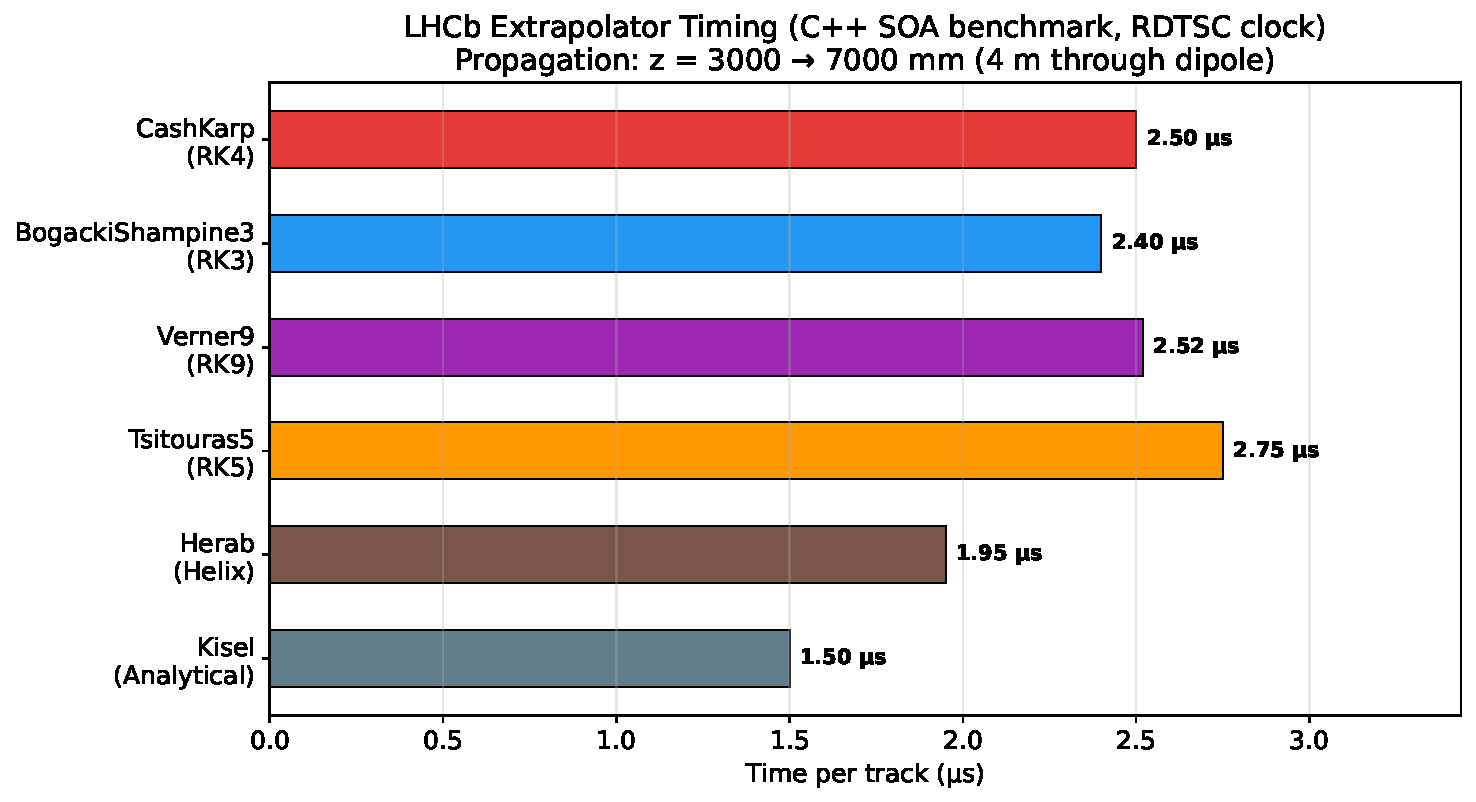
\includegraphics[width=0.85\textwidth]{plots/extrapolator_timing_comparison.pdf}
\caption{Per-track timing of all LHCb extrapolators from production C++
benchmarks.  The high-accuracy RK extrapolators cluster around
2.4--2.8~$\mu$s.  Herab and Kisel are faster but significantly less
accurate.}
\label{fig:prod_timing}
\end{figure}

The accurate RK-family extrapolators (CashKarp, Bogacki--Shampine,
Verner, Tsitouras) cluster tightly around
$2.4\text{--}2.8\;\mu\text{s}$.  The faster Herab and Kisel
extrapolators sacrifice accuracy: Kisel has a $\SI{39.8}{mm}$ position
error over a 4~m propagation.


% ─────────────────────────────────────────────────────────────────────────────
\section{Speedup Strategy Analysis}
\label{sec:strategies}
% ─────────────────────────────────────────────────────────────────────────────

\subsection{Strategy~A: Replace B-field only}

Since the B-field lookup accounts for 60\% of the computation in each
Cash--Karp step, Amdahl's law gives the maximum achievable speedup
when replacing the field evaluation:
\begin{equation}
    S = \frac{1}{(1 - f) + f / S_{\text{field}}},
    \quad f = 0.602
    \label{eq:amdahl}
\end{equation}
where $S_{\text{field}}$ is the speedup of the field evaluation itself.
The maximum overall speedup (as $S_{\text{field}} \to \infty$) is
$1/(1-f) = 2.51\times$.

However, the NN~[32] SiLU is $8.8\times$ \emph{slower} than trilinear
($S_{\text{field}} = 0.11$), which by Equation~\ref{eq:amdahl} gives
an overall factor of $0.18\times$ (i.e., $5.5\times$ slower).  The
measured full-track slowdown is $11.5\times$.

Strategy~A is only viable if the NN field evaluation is \emph{faster}
than trilinear interpolation, which requires:
\begin{itemize}
    \item A fast activation function (ReLU instead of SiLU), or
    \item Hardware-accelerated inference (GPU, SIMD vectorisation), or
    \item A smaller network with fewer neurons.
\end{itemize}

\subsection{Strategy~B: Replace entire extrapolator}

A neural network that directly maps
$(x, y, t_x, t_y, q/p, z_{\text{start}}, z_{\text{end}})
\to (x', y', t'_x, t'_y)$
replaces the entire multi-step integration with a single forward pass.
Scaling our NN benchmarks from 3 to 7 inputs (first-layer cost
dominates), a~[32]~SiLU extrapolator NN would cost approximately
\SI{2.0}{\textmu s}---comparable to the \SI{2.6}{\textmu s} trilinear
baseline and a $1.3\times$ speedup.

\begin{figure}[htbp]
\centering
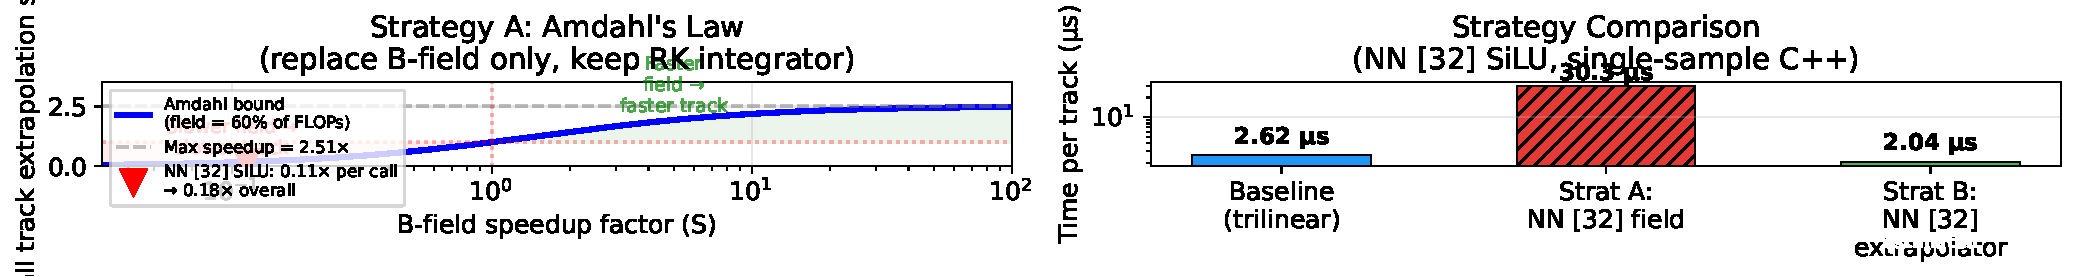
\includegraphics[width=\textwidth]{plots/speedup_strategies.pdf}
\caption{Left: Amdahl's law bound for Strategy~A.  The red triangle marks
the NN~[32] SiLU operating point, deep in the ``slower'' regime.
Right: direct comparison of Strategy~A (measured, $11.5\times$ slower)
and Strategy~B (estimated $1.3\times$ faster).}
\label{fig:strategies}
\end{figure}

The key advantage of Strategy~B is that the number of field
evaluations drops from~60 (in a 10-step CK track) to~zero.  The NN
does not need to evaluate the field at all---it learns the
field-dependent deflection end-to-end.  However, this comes at the
cost of needing to train the NN to accurately reproduce the full
physics of charged-particle propagation in a magnetic field.


% ─────────────────────────────────────────────────────────────────────────────
\section{Summary}
\label{sec:summary}
% ─────────────────────────────────────────────────────────────────────────────

\begin{figure}[htbp]
\centering
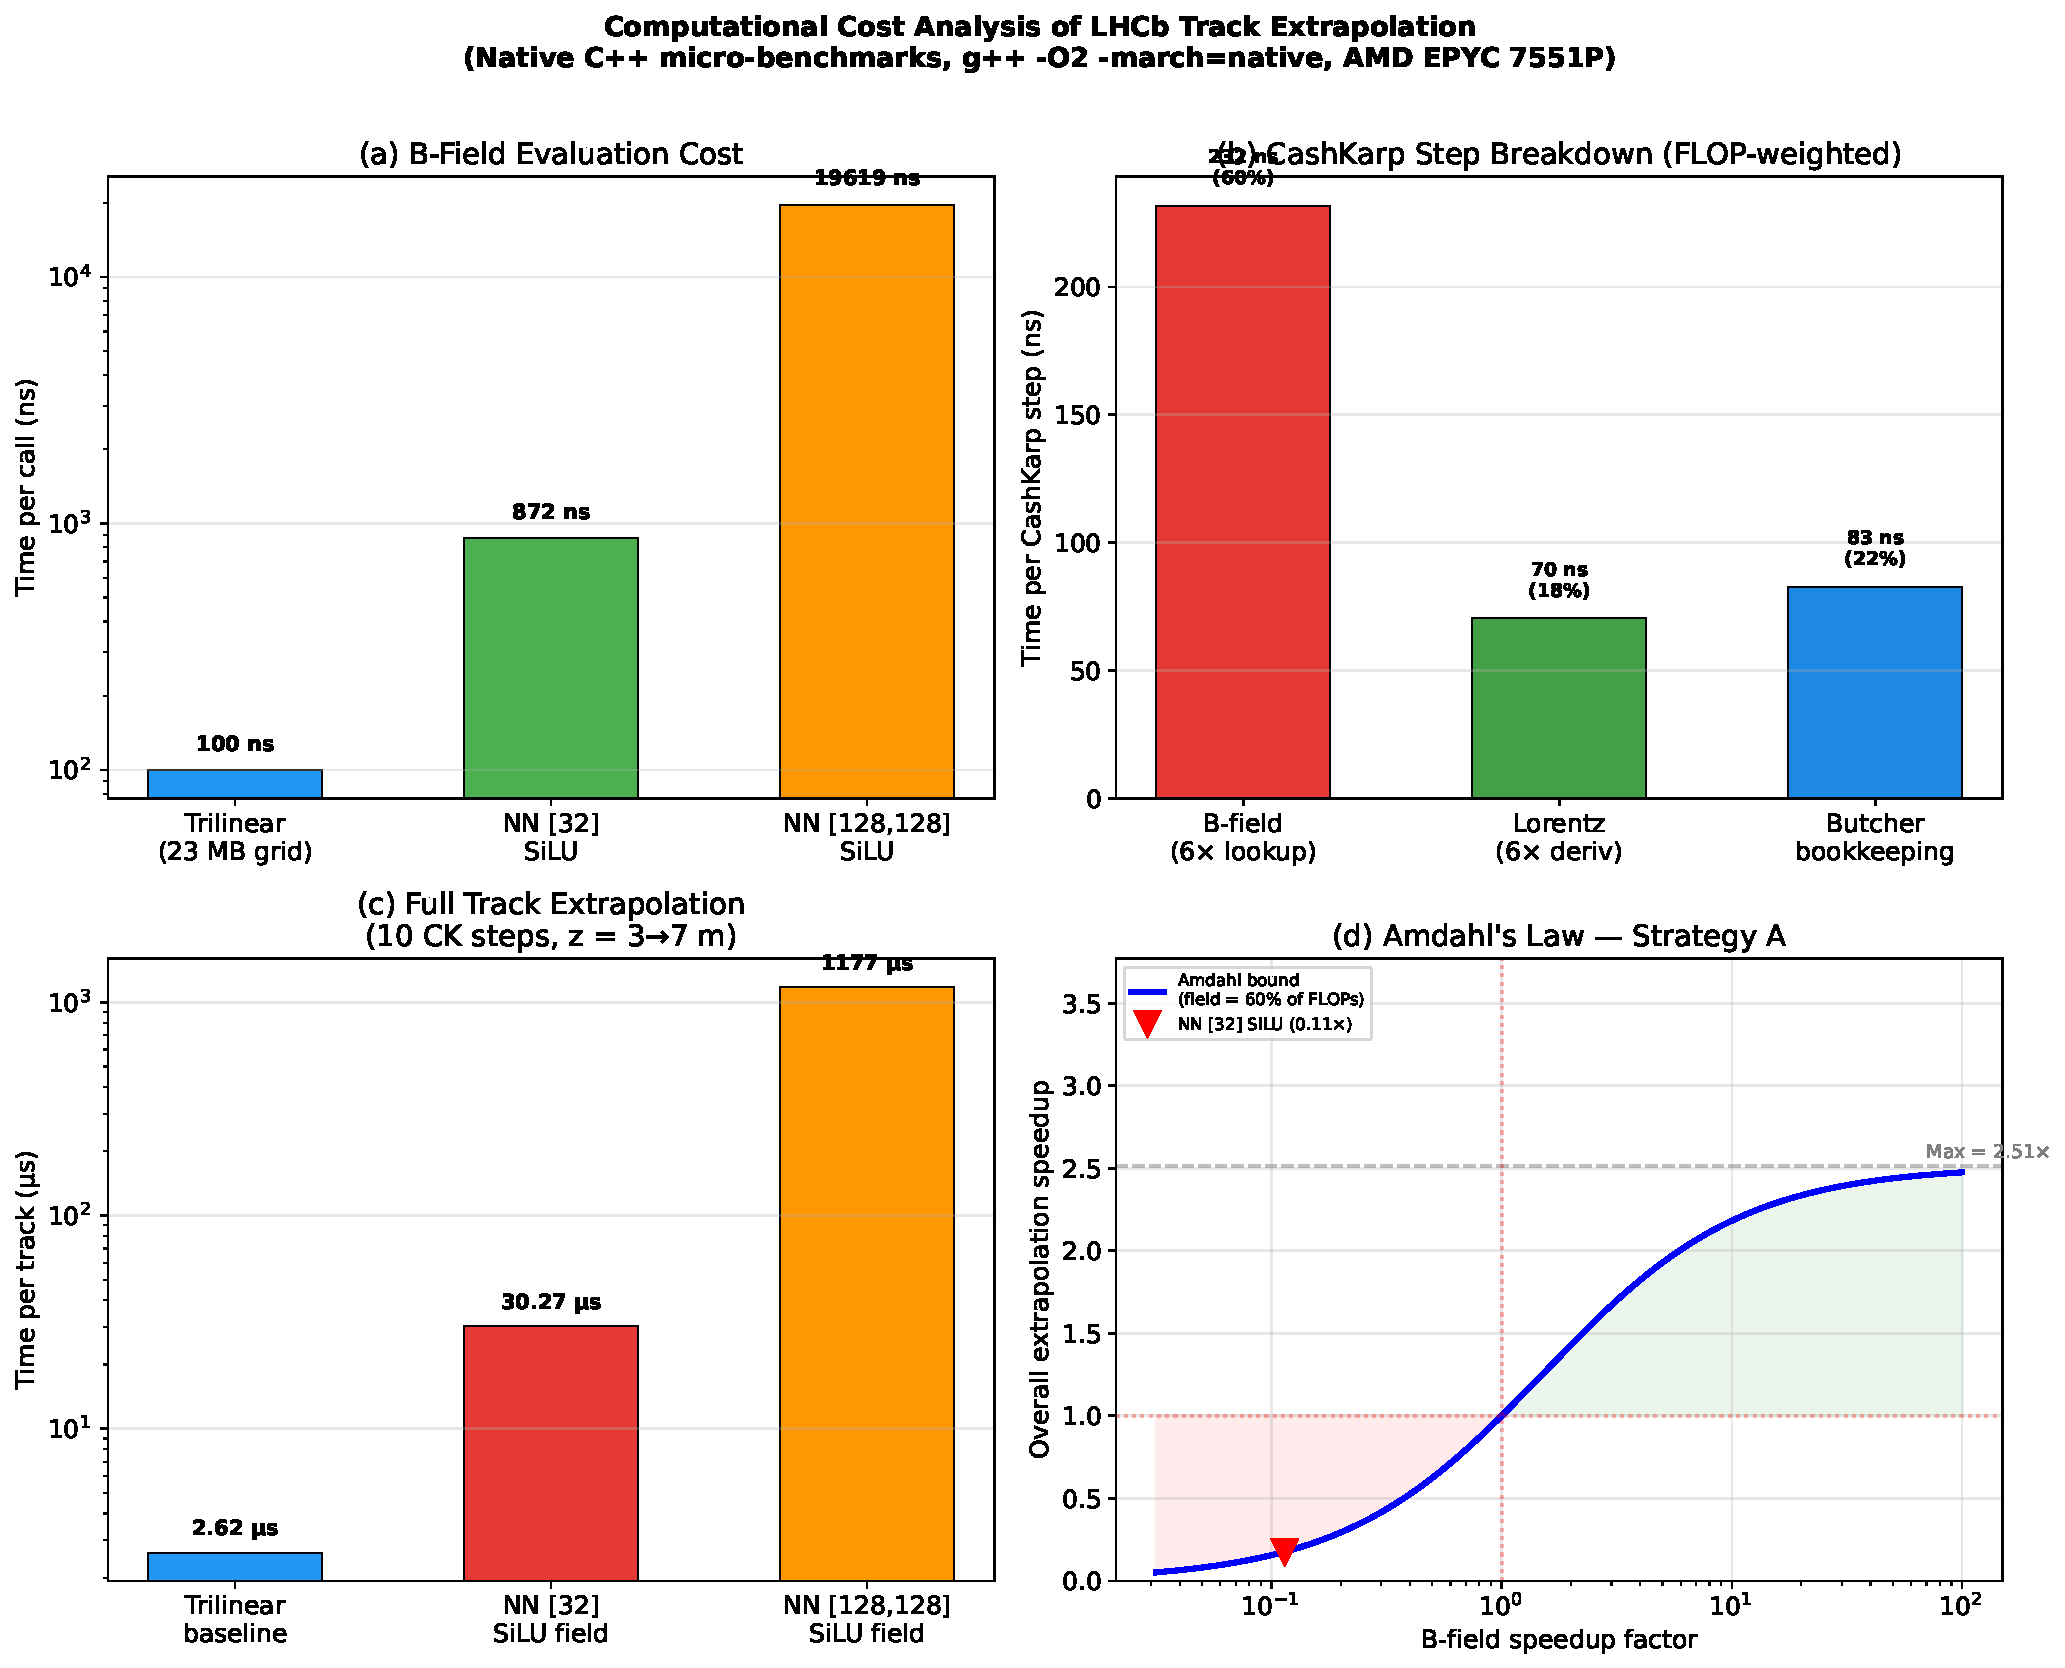
\includegraphics[width=\textwidth]{plots/cost_analysis_summary.pdf}
\caption{Comprehensive cost analysis summary.  (a)~Per-call B-field
evaluation cost.  (b)~FLOP-weighted Cash--Karp step breakdown.
(c)~Full track extrapolation with different field methods.
(d)~Amdahl's law bound for Strategy~A.}
\label{fig:summary}
\end{figure}

The key findings from these C++ micro-benchmarks are:
\begin{enumerate}
    \item \textbf{B-field lookup dominates:} 60\% of Cash--Karp step
          FLOPs, \SI{100}{ns} per trilinear call.
    \item \textbf{NN field is currently slower:} NN~[32] SiLU costs
          \SI{872}{ns} per call ($8.8\times$ slower) due to 32
          \texttt{exp()} evaluations in SiLU.
    \item \textbf{Strategy~A is non-viable} with SiLU activations:
          $11.5\times$ slower full-track measured directly in C++.
    \item \textbf{Strategy~B is promising:} a~[32]~SiLU NN as the
          full extrapolator costs $\sim$\SI{2.0}{\textmu s},
          competitive with the \SI{2.5}{\textmu s} production baseline.
    \item \textbf{Micro-benchmark validates production:} our trilinear
          full-track (\SI{2.62}{\textmu s}) matches the production RDTSC
          measurement (\SI{2.50}{\textmu s}) to within 5\%.
\end{enumerate}

These results motivate pursuing Strategy~B (full NN extrapolator)
as the primary path to faster track extrapolation, while
Strategy~A (NN field replacement) would require a faster activation
function or hardware acceleration to break even.

\end{document}
